\documentclass[a4paper,10pt]{article}
\usepackage[utf8]{inputenc}
\usepackage[MeX]{polski}
\usepackage{tikz}
\usepackage{url}
\usepackage{fullpage}
\usepackage{dirtree}
\usepackage{pgfplots}

\title{Grafy i Sieci. Sprawozdanie 3. \\ \small{SK11 Kolorowanie grafu za pomocą przeszukiwania z tabu.}}
\author{Michał Aniserowicz, Jakub Turek}
\date{}

\begin{document}

\maketitle

\section*{Temat projektu}

SK11 Kolorowanie grafu za pomocą przeszukiwania z tabu.

\section*{Uruchamianie programu}

Program uruchamiany jest z~linii poleceń. Aby go włączyć należy przejść do folderu z~projektem i~uruchomić polecenie \verb+python main.py <parametry>+. Podane \verb+<parametry>+ muszą być zgodne z~opcjami aplikacji:

\begin{verbatim}
main.py [-h] [-o output_file] [-v] -i maximum_iterations
-s maximum_iterations_without_score_change -m memory_size [--dimacs-compat]
input_file [input_file ...]
\end{verbatim}

Opis parametrów:

\begin{itemize}
    \item \verb+-h+ wyświetla pomoc do aplikacji (jest to treść zamieszczona powyżej).
    \item \verb+-o+ pozwala na przekierowanie wyjścia do pliku. Standardowo wszystkie komunikaty programu wypisywane są na konsoli. Podanie flagi \verb+-o output.txt+ spowoduje przekierowanie wyjścia programu do pliku \verb+output.txt+.
    \item \verb+-v+ jest opcjonalnym argumentem, który uruchamia tryb ,,rozmowny''\footnote{ang. verbose.}. W~tym trybie prezentowane są informacje o~poszczególnych iteracjach algorytmu (wraz z~wynikami iteracji, czasem wykonania i~zawartością pamięci ,,tabu''). W~trybie standardowym aplikacja przedstawia jedynie wynik działania programu.
    \item \verb+-i+ wymagany argument, który specyfikuje wielkość jednego z~kryteriów stopu: maksymalną liczbę iteracji. 
    \item \verb+-s+ wymagany argument, który specyfikuje wielkość jednego z~kryteriów stopu: maksymalną liczbę iteracji bez zmiany wyniku.
    \item \verb+-m+ wymagany argument, który specyfikuje rozmiar pamięci ,,tabu''.
    \item \verb+--dimacs-compat+ opcjonalna flaga, która pozwala na czytanie danych z~plików w~formacie DIMACS\footnote{\url{http://mat.gsia.cmu.edu/COLOR/general/ccformat.ps}.}. Standardowo program obsługuje wejście we właściwym dla siebie formacie.
    \item \verb+input_file+ specyfikuje nazwę pliku wejściowego, który zawiera definicję grafu, na którym przeprowadzone zostaną obliczenia. Plików wejściowych może być wiele, natomiast wymagany jest przynajmniej jeden.
 \end{itemize}

\noindent Przykładowe wywołanie programu:

\begin{verbatim}
python main.py -v -o queen6_6_mem01.txt --dimacs-compat -i 200 -s 50 -m 5 queen6_6.txt
\end{verbatim}

\noindent Powyższe wywołanie programu uruchamia aplikację w~trybie ,,rozmownym'', przekierowuje wyjście programu do pliku \verb+queen6_6_mem01.txt+, pobiera dane z~pliku \verb+queen6_6.txt+ w~formacie DIMACS i~uruchamia aplikację dla maksymalnie dwustu iteracji, pięćdziesięciu iteracji bez zmiany wyniku oraz rozmiarem pamięci ,,tabu'' równym pięć.

\section*{Poszukiwanie optymalnego rozmiaru ,,tabu''}

Przy poszukiwaniu optymalnego rozmiaru tabu zostały przeprowadzone dwa badania:

\begin{enumerate}
    \item Badanie czasu obliczeń. Dla dwóch grafów, dla których znane jest optymalne kolorowanie, przeprowadzono pomiar czasu wyznaczania poprawnego kolorowania dla identycznych kryteriów stopu. Kryteria stopu były dobrane w~taki sposób, aby wygaszanie algorytmu było powodowane przez osiągnięcie maksymalnej liczby iteracji bez zmiany rezultatu. Pod uwagę brane były wyłącznie próby, które kończyły się poprawnym obliczeniem rozwiązania.
    \item Badanie poprawności obliczeń. Dla grafu, dla którego znane jest optymalne kolorowanie, przeprowadzono pomiar prawdopodobieństwa poprawnego obliczenia rezultatu dla identycznych kryteriów stopu.
\end{enumerate}

\noindent W~obu przypadkach początkowe pokolorowanie grafu dobierane było w~sposób losowy. Wyniki ilustrują poniższe wykresy:

\begin{figure}[ht!]
    \centering
    \begin{tikzpicture}
        \begin{axis}[xlabel=Rozmiar pamięci,ylabel=Czas, xtick={1, 2, 3, 4, 5, 6, 7, 8, 9, 10, 11, 12, 13, 14, 15, 16, 17, 18, 19, 20}, width=.8\textwidth]
        \addplot coordinates {
            (1, 216.103834867)
            (2, 153.564208031)
            (3, 144.054646015)
            (4, 121.636734009)
            (5, 102.596985817)
            (6, 92.7162508965)
            (7, 109.012079954)
            (8, 85.7409420013)
            (9, 85.9665899277)
            (10, 81.3143780231)
            (11, 66.0520329475)
            (12, 139.750561953)
            (13, 103.690033913)
            (14, 69.9469909668)
            (15, 60.0240390301)
            (16, 94.9388859272)
            (17, 96.8258011341)
            (18, 70.6327459812)
            (19, 55.1863398552)
            (20, 42.0572459698)
        };
        \addplot coordinates {
            (1, 14.0370841026)
            (2, 17.6206011772)
            (3, 13.3633220196)
            (4, 17.4316580296)
            (5, 12.6170749664)
            (6, 13.7205200195)
            (7, 14.5897459984)
            (8, 13.8318810463)
            (9, 14.302770853)
            (10, 13.5634422302)
            (11, 18.363656044)
            (12, 16.7718977928)
            (13, 14.5919039249)
            (14, 15.4569129944)
            (15, 14.760160923)
            (16, 17.1893560886)
            (17, 13.0198259354)
            (18, 12.3857138157)
            (19, 20.1795430183)
            (20, 12.964715004)
        };
        \legend{Duży graf, Mały graf}
        \end{axis}
    \end{tikzpicture}
    \caption{Czas wykonania algorytmu w~zależności od rozmiaru pamięci.}
    \label{fig:tabu_size_execution_time}
\end{figure}
            
\begin{figure}[ht!]
    \centering
    \begin{tikzpicture}
        \begin{axis}[xlabel=Rozmiar pamięci,ylabel=Prawdopodobieństwo uzyskania optymalnego wyniku w~10 próbach, xtick={1, 2, 3, 4, 5, 6, 7, 8, 9, 10, 11, 12, 13, 14, 15, 16, 17, 18, 19, 20}, width=.8\textwidth]
        \addplot coordinates {
            (1, 0.6)
            (2, 0.8)
            (3, 0.8)
            (4, 0.5)
            (5, 0.7)
            (6, 0.7)
            (7, 0.9)
            (8, 0.8)
            (9, 0.8)
            (10, 0.9)
            (11, 0.8)
            (12, 0.9)
            (13, 0.9)
            (14, 0.8)
            (15, 0.8)
            (16, 0.8)
            (17, 0.9)
            (18, 0.8)
            (19, 0.7)
            (20, 0.9)
        };
        \end{axis}
    \end{tikzpicture}
    \caption{Optymalność wyniku w~zależności od rozmiaru pamięci.}
    \label{fig:tabu_size_optimal_coloring}
\end{figure}

Analizując rysunki \ref{fig:tabu_size_execution_time} oraz \ref{fig:tabu_size_optimal_coloring} możemy wyciągnąć następujące wnioski:

\begin{itemize}
    \item Dla dużego grafu i~małych rozmiarów pamięci ,,tabu'' czas wykonywania algorytmu jest znacznie dłuższy niż dla większych rozmiarów.
    \item Dla dużego grafu czas wykonywania algorytmu drastycznie maleje dla rozmiarów ,,tabu'' z~przedziału $[1; 6]$. Dla większych rozmiarów pamięci krzywa czasu wykonania programu nie jest monotoniczna. Dla tych rozmiarów pamięci istotniejszy jest czynnik związany z~początkowym pokolorowaniem grafu.
    \item Analiza czasu wykonania algorytmu dla małego grafu nie daje nam żadnych dodatkowych informacji. Dla testowanego grafu czasy wykonywania programu były zbliżone dla każdej wielkości pamięci ,,tabu''.
    \item Analiza prawdopodobieństwa uzyskania optymalnego wyniku pozwala stwierdzić, że optymalnym rozmiarem pamięci ,,tabu'' jest 7. Powyżej tego progu średnie prawdopodobieństwo uzyskania optymalnego wyniku wynosi 83,57\%. Poniżej tego progu średnie prawdopodobieństwo uzyskania optymalnego wyniku wynosi 68,33\%.
\end{itemize}

\section*{Badanie wydajności algorytmu}

\begin{figure}[ht!]
    \centering
    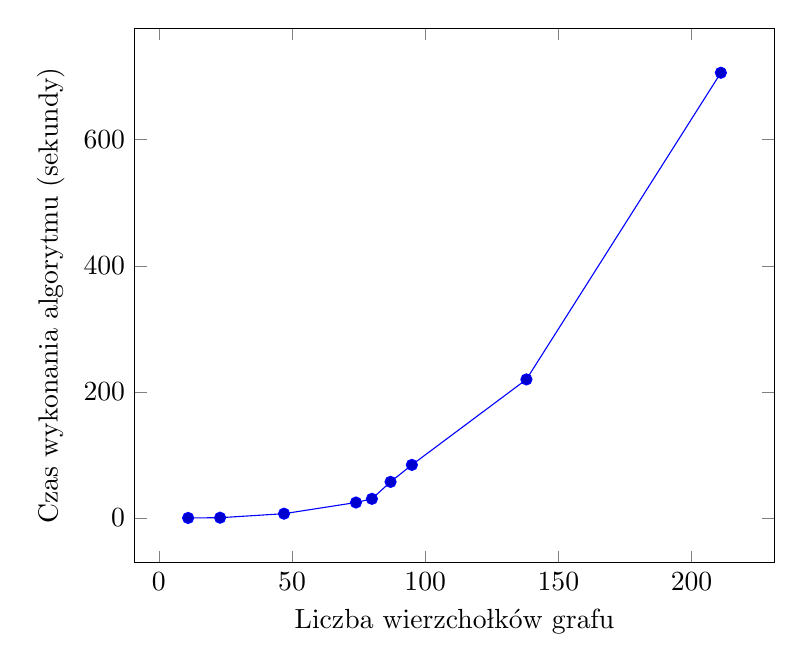
\begin{tikzpicture}
        \begin{axis}[xlabel=Liczba wierzchołków grafu,ylabel=Czas wykonania algorytmu (sekundy), width=.8\textwidth]
        \addplot coordinates {
            (11, 0.0313858985901)
            (23, 0.416062116623)
            (47, 6.79242110252)
            (74, 24.5025429726)
            (80, 30.3272099495)
            (87, 57.2853310108)            
            (95, 84.1847200394)
            (138, 219.825026989)
            (211, 706.329546928)
        };
        \end{axis}
    \end{tikzpicture}
    \caption{Czas wykonania algorytmu w~zależności od liczby wierzchołków grafu.}
    \label{fig:algorithm_efficiency}
\end{figure}

Wydajność algorytmu została zmierzona dla optymalnego rozmiaru pamięci ,,tabu'' wyznaczonego we wcześniejszej części raportu (7). Testy zostały przeprowadzone na grafach, dla których znane jest optymalne pokolorowanie. Pozostałe parametry algorytmu zostały dobrane tak, aby odnaleźć optymalne pokolorowanie.
    
Zgodnie z~przewidywaniami w~raporcie drugim, z~wykresu \ref{fig:algorithm_efficiency} wynika, że algorytm ma złożoność czasową wykładniczą.

Zwiększenie wydajności aplikacji byłoby możliwe poprzez zmianę algorytmu poruszania się po grafie. Wykorzystany w~projekcie DFS można zastąpić zwykłą iteracją po liście, która będzie uporządkowana np. według rosnących identyfikatorów wierzchołków.

\section*{Poprawność algorytmu}

Program został stworzony przy użyciu techniki TDD\footnote{Test-Driven Development. Technika programowania, w~której programista najpierw tworzy automatyczne testy jednostkowe do danej funkcjonalności, a~następnie implementuje właściwą funkcjonalność.}, co zapewnia poprawność implementacji algorytmu. Kod odpowiedzialny za algorytm jest pokryty testami jednostkowymi niemalże w~100\%.

Poza testami jednostkowymi aplikacja była testowana dla grafów o~określonym optymalnym pokolorowaniu, zaczerpniętych ze strony \url{http://mat.gsia.cmu.edu/COLOR/instances.html}. Algorytm przeszedł testy dla następujących zbiorów danych:

\begin{itemize}
    \item \verb+zeroin.i.1.col+, \verb+zeroin.i.2.col+, \verb+zeroin.i.3.col+,
    \item \verb+anna.col+, \verb+david.col+, \verb+huck.col+, \verb+jean.col+,
    \item \verb+games120.col+,
    \item \verb+queen5_5.col+,
    \item \verb+myciel3.col+, \verb+myciel4.col+, \verb+myciel5.col+, \verb+myciel6.col+, \verb+myciel7.col+.
\end{itemize}

Dla każdego z~grafów z~powyższych zbiorów danych udało się znaleźć takie wartości kryteriów stopu, żeby dla optymalnej wielkości pamięci ,,tabu'' aplikacja odnalazła prawidłowe pokolorowanie, które jest optymalne (optymalność stwierdzana była na podstawie danych znajdujących się w~przytoczonym zbiorze danych). 

\section*{Wnioski}

Algorytm przeszukiwania przestrzeni z~,,tabu'' jest wydajnym algorytmem poszukiwania jak najbardziej optymalnego pokolorowania grafu. Dzięki zastosowaniu pamięci krótkoterminowej algorytm dobrze radzi sobie z~opuszczaniem lokalnych minimów dla zdefiniowanej funkcji celu. Pamięć ,,tabu'' pozwala również ograniczyć czas niezbędny do przeprowadzenia obliczeń. Iteracyjna natura algorytmu sprawia, że jest on dobrze skalowalny - pozwala na wyznaczenie suboptymalnego rozwiązania w~krótkim czasie.

Problemem algorytmu kolorowania grafu z~,,tabu'' jest zdefiniowanie i~wyznaczanie wartości konfiguracyjnych kryteriów stopu. Nie da się wyznaczyć uniwersalnej miary, która będzie właściwa dla wszystkich typów i~rozmiarów grafów. W~trakcie badań przeprowadzanych na potrzeby projektu wielokrotnie zdarzały się sytuacje, gdy zadane kryteria stopu powodowały zbyt szybkie zakończenie algorytmu. Konsekwencją tego była konieczność ponownego wykonywania obliczeń. Z~tego powodu algorytm nie może być stosowany do wyznaczania optymalnego pokolorowania, jeżeli nie znamy z~góry liczby barw, które składają się na to kolorowanie. Pozwala on natomiast łatwo wyznaczyć kolorowanie grafu $n$~kolorami, jeżeli takie pokolorowanie istnieje.

Ze względu na brak jasno określonych kryteriów stopu i~ich wielkości algorytm wyznaczania kolorowania grafu z~,,tabu'' mógłby znaleźć zastosowanie w~systemie typu \emph{supervised}. Decyzję o~zakończeniu algorytmu podejmowałby nadzorca systemu na podstawie jakości wyniku uzyskanego na wyjściu $i$-tej iteracji.

W~ramach badań przeprowadzonych w~trakcie projektu udało się wyznaczyć uniwersalny rozmiar pamięci ,,tabu'', który może być wykorzystywany dla różnych rozmiarów i~typów grafów.

Przeprowadzone badania dowodzą, że szybkość i~skuteczność działania algorytmu jest ściśle związana ze wstępnym pokolorowaniem grafu. Wstępne kolorowanie ma znaczący wpływ na liczbę iteracji algorytmu potrzebnych do wyznaczenia pokolorowania optymalnego, co rzutuje na konfigurację kryteriów stopu, które używane są do konkretnego typu grafu.

\section*{Dokumentacja kodu źródłowego}

Kod źródłowy projektu został stworzony w~języku Python. Program jest kompatybilny z~wersją \verb+2.7.x+ interpretera. Aplikacja testowana była w~Pythonie w~wersji \verb+2.7.5+, pod kontrolą systemu \verb+OS X 10.9+ (\verb+Mavericks+). Do uruchomienia testów jednostkowych wymagane jest zainstalowanie biblioteki \verb+Mock+\footnote{Biblioteka została wcielona do specyfikacji języka począwszy od wersji 3.3.} w~wersji \verb+1.0.1+.

Ogólna struktura kodu źródłowego została przedstawiona na poniższym diagramie.

\dirtree{%
 .1 /.
 .2 aspiration\_criteria.
 .3 aspiration\_criteria.py.
 .2 evaluation.
 .3 cost\_evaluator.py. 
 .2 graph.
 .3 graph\_cloner.py.
 .3 node.py.
 .3 node\_iterator.py.
 .2 input.
 .3 dimacs\_input\_reader.py.
 .3 input\_reader.py.
 .3 input\_reader\_factory.py.
 .2 memory.
 .3 memory.py.
 .2 permutation.
 .3 color\_permutator.py.
 .3 fast\_color\_permutator.py.
 .2 progress.
 .3 progress\_writer.py.
 .2 search.
 .3 search\_performer.py.
 .2 stop\_criteria.
 .3 stop\_criteria.py.
 .2 test.
 .3 ....
 .2 validation.
 .3 coloring\_validator.py.
 .3 connection\_validator.py.
 .2 main.py.
}
 
\subsection*{Reprezentacja grafu}

Graf reprezentowany jest z~wykorzystaniem klasy \verb+Node+ reprezentującej wierzchołek. Ponieważ, z~założenia, aplikacja operuje wyłącznie na grafach spójnych nie ma znaczenia, od którego wierzchołka rozpoczynamy analizę struktury.

\noindent\begin{table}[ht!]
            \begin{tabular}{lr}
                \begin{minipage}[t]{0.55\textwidth}
                    \begin{verbatim}
class Node:
  Id = 0

  def __init__(self, color=None, 
    node_id=None, previous_color=None):
    
    self.edges = []
    self.color = color

    if node_id is not None:
      self.node_id = node_id
    else:
      self.node_id = Node.Id
      Node.Id += 1

    self.previous_color = self.color

    if previous_color is not None:
      self.previous_color = previous_color

  def add_edges(self, nodes):
    for node in nodes:
      if node not in self.edges:
        self.edges.append(node)

      if self not in node.edges:
        node.edges.append(self)

  def iterator(self):
    return NodeIterator(self)

  def get_node_of_id(self, node_id):
    for node in self.iterator():
      if node.node_id == node_id:
        return node

  def node_count(self):
    return sum(1 for _ in self.iterator())

  def get_colors_count(self):
    colors = set()

    for node in self.iterator():
      colors.add(node.color)

    return len(colors)
                    \end{verbatim}
                \end{minipage}
                
                &
        
                \begin{minipage}[t]{0.45\textwidth}
                    \noindent Metoda \verb+init+ służy do konstrukcji węzła. Węzeł posiada następujące składowe:
                    \begin{itemize}
                        \item \verb+edges+ lista wierzchołków połączonych z~danym węzłem,
                        \item \verb+color+ kolor wierzchołka,
                        \item \verb+node_id+ identyfikator wierzchołka,
                        \item \verb+previous_color+ poprzedni kolor wierzchołka używany do wyznaczania permutacji.
                    \end{itemize}
\\
                    
                    \noindent Identyfikator, jak również kolor wierzchołka, mogą być dowolnego typu (liczba, ciąg znaków...). Identyfikatory mogą, ale nie muszą być nadawane automatycznie - są wtedy typu liczbowego. Kolejne identyfikatory pobierane są ze zmiennej ,,statycznej'' \verb+Id+. \\ \\
                    
                    \noindent Metoda \verb+add_edges+ pozwala na łączenie wierzchołka z~innymi wierzchołkami. Implementacja została przygotowana dla grafów nieskierowanych, a~więc podczas dodawania krawędzi tworzone jest od razu wiązanie dwustronne. \\ \\ \\
                                        
                    \noindent Do poruszania się po grafie wykorzystywany jest iterator, który korzysta z~algorytmu DFS. \\
                    
                    \noindent Metoda \verb+get_node_of_id+ pozwala na dojście do dowolnego wierzchołka po identyfikatorze. \\ \\ \\
                    
                    \noindent Metoda \verb+node_count+ zlicza liczbę wierzchołków w~grafie. \\
                    
                    \noindent Metoda \verb+get_colors_count+ zwraca liczbę kolorów, którymi w~chwili obecnej pokolorowany jest graf.
                                        
                \end{minipage}
            
                \\
            
            \end{tabular}
        
        \end{table}
        
Klasa \verb+NodeIterator+ dostarcza interfejs iteratora dla wierzchołka grafu. Udostępnia ona metodę \verb+next+, która dla danego wierzchołka zwraca kolejny w~porządku przeszukiwania w~głąb. Przeszukiwanie w~głąb oznacza, że w~pierwszej kolejności przechodzimy do pierwszego dziecka danego wierzchołka, a~dopiero po powrocie algorytmu do tego samego wierzchołka przeglądamy jego kolejne dziecko. Wykorzystanie wzorca iteratora pozwala na przeglądanie grafu w~wygodny sposób - używając do tego pętli \verb+for+.

Oprócz narzędzia do przeglądania grafu zaimplementowana została też metoda do kopiowania całego grafu. Jest ona zawarta w~metodzie \verb+clone+ klasy \verb+GraphCloner+. Klonowanie grafu jest przydatne podczas wyznaczania możliwych permutacji kolorów. Wystarczy powielić cały graf i~zmienić barwę analizowanego wierzchołka.

\subsection*{Funkcja kosztu}

\noindent\begin{table}[ht!]
            \begin{tabular}{lr}
                \begin{minipage}[t]{0.55\textwidth}
                    \begin{verbatim}
class CostEvaluator:
  def evaluate(root_node, color_set):
    c, e = self.evaluate_score_for_colors(
      root_node)
    return self.evaluate_cost(color_set, c, e)

  def evaluate_score_for_colors(root_node):
    inspected_edges, c, e = [], {}, {}

    for node in root_node.iterator():
      if node.color not in c:
        c[node.color] = 0

      c[node.color] += 1

      for child_node in node.edges:
        if {node, child_node} not in 
            inspected_edges and 
            color == child_node.color:
          if node.color not in e:
            e[node.color] = 0

          e[node.color] += 1
          
          inspected_edges.append(
            {node, child_node})

    return c, e
    
  def evaluate_cost(color_set, c, e):
    cost = 0

    for color in color_set:
      c_i, e_i = 0, 0

      if color in c:
        c_i = c[color]
      if color in e:
        e_i = e[color]

      cost += -1 * c_i ** 2 + 2 * c_i * e_i

    return cost
                    \end{verbatim}
                \end{minipage}
                
                &
        
                \begin{minipage}[t]{0.45\textwidth}
                    \noindent Metoda \verb+evaluate+ oblicza wartość funkcji kosztu dla danego grafu. Algorytm wykonywany jest w~dwóch krokach. \\ \\ \\
                    
                    \noindent W~pierwszym kroku obliczane są wartości $C_{i}$ oraz $E_{i}$ dla każdego koloru. Metoda \verb+evaluate_score_for_colors+ wykonuje niezbędne obliczenia. Istotne jest, że wszystkie wartości wyznaczane są w~czasie pojedynczego przejścia przez graf, dzięki czemu metoda jest wydajna. \\ \\ \\ \\ \\ \\ \\ \\ \\ \\ \\ \\ \\ \\ \\ \\
                    
                    \noindent Następnie zliczane są wyniki dla wszystkich kolorów znajdujących się w~zbiorze. Funkcja \verb+evaluate_cost+ oblicza wartość na podstawie wzoru $f(G) = -\sum_{i=1}^{k} C_i^2 + \sum_{i=1}^{k} 2 C_i E_i$, gdzie $C_{i}$ oznacza liczbę wierzchołków o~kolorze $i$, natomiast $E_{i}$ oznacza liczbę krawędzi, która łączy dwa wierzchołki o~kolorze $i$. \\
                \end{minipage}
            
                \\
            
            \end{tabular}
        
        \end{table}
        
Ponadto klasa \verb+CostEvaluator+ posiada metodę \verb+evaluate_score_for_permutation+. Pozwala ona na szybkie obliczanie funkcji celu dla permutacji pokolorowania grafu. Metoda przyjmuje parametry:

\begin{itemize}
    \item \verb+node+ wierzchołek, którego kolorowanie ulegnie zmianie w~trakcie permutacji.
    \item \verb+target_color+ docelowy kolor dla wierzchołka (po permutacji).
    \item \verb+base_c+ słownik wartości $C_{i}$ przed wykonaniem permutacji.
    \item \verb+base_e+ słownik wartości $E_{i}$ przed wykonaniem permutacji.
    \item \verb+color_set+ zbiór wszystkich kolorów.
\end{itemize}

\noindent Korzystając z~powyższych parametrów metoda wyznacza funkcję kosztu dokonując pojedynczego przejścia po wierzchołku oraz wszystkich jego sąsiadach, a~nie po całym grafie. Pozwala to znacząco zredukować czas szacowania funkcji kosztu dla permutacji.

\subsection*{Pamięć}

\noindent\begin{table}[ht!]
            \begin{tabular}{lr}
                \begin{minipage}[t]{0.55\textwidth}
                    \begin{verbatim}
class Memory:
  def __init__(self, short_term_memory_size):
    self.memory = []
    self.short_term_memory_size = 
      short_term_memory_size

  def add_to_memory(self, node, color):
    self.memory.append((node.node_id, color))

  def clear_memory(self):
    self.memory = []

  def get_short_term_memory(self):
    return self.memory[
      -self.short_term_memory_size:]
    
  def get_long_term_memory(self):
    return self.memory

  def is_in_short_term_memory(self, node, color):
    return (node.node_id, color) in 
      self.get_short_term_memory()

  def is_in_long_term_memory(self, node, color):
    return (node.node_id, color) in 
      self.get_long_term_memory()
                    \end{verbatim}
                \end{minipage}
                
                &
        
                \begin{minipage}[t]{0.45\textwidth}
                    \noindent Klasa \verb+Memory+ realizuje pamięć poprzez przechowywanie par $(id_{wierzchołka}, kolor)$ w~liście \verb+memory+. Pamięć krótkoterminowa i~długoterminowa jest realizowana z~wykorzystaniem jednej pamięci fizycznej. \\ 
                    
                    \noindent Dodanie wpisu do pamięci polega na dopisaniu pary $(id_{wierzchołka}, kolor)$ na końcu pamięci. \\ 
                    
                    \noindent Metoda \verb+clear_memory+ czyści zawartość pamięci. \\
                    
                    \noindent Pamięć krótkoterminowa to $n$ ostatnich wpisów listy, gdzie $n$ to rozmiar tabu i~jest definiowany zmienną \verb+short_term_memory_size+. \\
                    
                    \noindent Pamięć długoterminowa to cała zawartość pamięci. \\
                    
                    \noindent Metoda \verb+is_in_short_term_memory+ sprawdza, czy dana kombinacja znajduje się w~pamięci krótkoterminowej. \\
                    
                    \noindent Metoda \verb+is_in_long_term_memory+ oferuje analogiczną funkcjonalność dla pamięci długoterminowej.
                \end{minipage}
            
                \\
            
            \end{tabular}
        
        \end{table}

\subsection*{Kryteria stopu}

Zgodnie z~założeniami przedstawionymi w~poprzednich raportach zaimplementowane zostały dwa kryteria stopu:

\begin{itemize}
    \item maksymalna liczba iteracji,
    \item maksymalna liczba iteracji bez zmiany najlepszego wyniku.
\end{itemize}

\noindent\begin{table}[ht!]
            \begin{tabular}{lr}
                \begin{minipage}[t]{0.55\textwidth}
                    \begin{verbatim}
class StopCriteria:
  def __init__(self, max_iters, 
      max_iters_without_change):
    self.max_iters = max_iters
    self.max_iters_without_change = 
      max_iters_without_change
    self.current_iters = 0
    self.current_iters_without_change = 0
    self.previous_score = None

  def reset(self):
    self.current_iters = 0
    self.current_iters_without_change = 0
    self.previous_score = None

  def next_iteration(self, score):
    self.current_iters += 1

    if self.previous_score is None or 
        self.previous_score != score:
      self.previous_score = score
      self.current_iters_without_change = 1
    else:
      self.current_iters_without_change += 1

  def should_stop(self):
    return self.current_iters >= self.max_iters 
      or self.current_iters_without_change >= 
        self.max_iters_without_change
                    \end{verbatim}
                \end{minipage}
                
                &
        
                \begin{minipage}[t]{0.45\textwidth}
                    \noindent Klasa \verb+StopCriteria+ realizuje kryteria stopu. Zlicza ona liczbę iteracji algorytmu oraz liczbę iteracji bez zmiany wyniku i~porównuje je z~wartościami konfiguracyjnymi ze zmiennych \verb+max_iters+ oraz \verb+max_iters_without_change+. \\ \\ \\ \\ \\ \\ \\ \\ \\ \\ 
                    
                    \noindent Metoda \verb+next_iteration+ jest wywoływana przy każdej iteracji przeszukiwania z~tabu. Parametrem tej metody jest najlepsza znaleziona wartość funkcji celu. Funkcja sprawdza czy oszacowanie uległo zmianie. \\ \\ \\ \\ \\
                    
                    \noindent Metoda \verb+should_stop+ orzeka czy wykonywanie algorytmu powinno zakończyć się na podstawie kryteriów stopu. \\
                \end{minipage}
            
                \\
            
            \end{tabular}
        
        \end{table}
        
\subsection*{Kryteria aspiracji}

Kryteria aspiracji orzekają, kiedy wolno pominąć restrykcje ,,tabu''. Zaimplementowane zostało proste kryterium aspiracji, które pomija restrykcje ,,tabu'' wtedy i~tylko wtedy, gdy dana permutacja posiada lepsze oszacowanie funkcji celu niż najlepsze dotychczas odnalezione.

\noindent\begin{table}[ht!]
            \begin{tabular}{lr}
                \begin{minipage}[t]{0.55\textwidth}
                    \begin{verbatim}
class AspirationCriteria:
  def __init__(self, banned_trans, best_score):
    self.banned_trans = banned_trans
    self.best_score = best_score


  def is_allowed(self, node, color, cost):
    if (node.node_id, color) not in 
        self.banned_trans:
      return True

    return self.best_score is not None and 
      cost < self.best_score
                    \end{verbatim}
                \end{minipage}
                
                &
        
                \begin{minipage}[t]{0.45\textwidth}
                    \noindent Klasa \verb+AspirationCriteria+ orzeka czy należy wziąć pod uwagę restrykcje ,,tabu''. Przechowuje listę zabronionych przejść \verb+banned_trans+ oraz najlepszy znaleziony wynik funkcji celu \verb+best_score+. \\
                    
                    \noindent Metoda \verb+is_allowed+ stwierdza czy wolno dokonać dane przejście w~permutacji. Jeżeli przejście nie jest objęte restrykcją ,,tabu'' to zawsze można dokonać tego przejścia. W~przeciwnym wypadku można go dokonać tylko wtedy, gdy oszacowanie funkcji celu dla permutacji jest lepsze niż najlepsze znalezione dotychczas oszacowanie.
                \end{minipage}
            
                \\
            
            \end{tabular}
        
        \end{table}

\subsection*{Weryfikacja pokolorowania}

\noindent\begin{table}[ht!]
            \begin{tabular}{lr}
                \begin{minipage}[t]{0.55\textwidth}
                    \begin{verbatim}
class ColoringValidator:
  def is_coloring_valid(root_node):
    for node in root_node.iterator():
      for child_node in node.edges:
        if node.color == child_node.color:
          return False

    return True
                    \end{verbatim}
                \end{minipage}
                
                &
        
                \begin{minipage}[t]{0.45\textwidth}
                    \noindent Metoda \verb+is_coloring_valid+ klasy \verb+ColoringValidator+ sprawdza czy w~grafie nie istnieje krawędź łącząca dwa wierzchołki identycznego koloru.
                \end{minipage}
            
                \\
            
            \end{tabular}
        
        \end{table}
        
\subsection*{Wyznaczanie permutacji pokolorowań}

Wyznacznie permutacji pokolorowań to część algorytmu, która wymagała największej optymalizacji. W~przypadku podejścia naiwnego, które polegało na wyznaczeniu wszystkich możliwych sąsiedztw, a~następnie oszacowania dla nich wartości funkcji celu, pojedyncze iteracje przeszukiwania z~,,tabu'' (nawet dla stosunkowo małego grafu) trwały około 20 sekund.

Optymalizacja polegała na spostrzeżeniu, że do poprawnego działania algorytmu nie jest potrzebna pełna informacja o~całym możliwym sąsiedztwie. W~kolejnym kroku algorytmu odcinane były bowiem wszystkie permutacje, które w~danej iteracji nie uzyskały maksymalnej wartości funkcji celu. Optymalizacja została dokonana poprzez złączenie ze sobą dwóch kroków algorytmu:

\begin{itemize}
    \item Dla każdej badanej permutacji od razu dokonywane jest obliczanie wartości funkcji celu. Można zrobić to w~bardzo wydajny sposób. Przed dokonaniem permutacji należy jednokrotnie obliczyć wartość funkcji celu dla całego grafu i~zachować cząstkowe wartości $C_{i}$ oraz $E_{i}$ dla wszystkich kolorów. Następnie, po wykonaniu permutacji koloru jednego wierzchołka, należy przeanalizować w~jaki sposób zmiana ta wpłynęła na wartość funkcji celu. Ponieważ permutacja ma zasięg lokalny, wystarczy zbadać wyłącznie sąsiadów analizowanego wierzchołka, a~nie cały graf.
    \item Badając każde kolejne sąsiedztwo przechowujemy informację o~wartości funkcji celu dla najlepszej znalezionej do tej pory permutacji. Jeżeli obliczona dla nowej permutacji wartość funkcji celu jest gorsza niż dla już znalezionej, odrzucamy takie sąsiedztwo. W~przypadku, gdyby wartości okazały się identyczne, należy dopisać kolejną permutację do listy zwracanych wartości, a~gdyby nowa permutacja okazała się najlepsza, należy wyczyścić listę pozostałych i~wstawić w~ich miejsce wyłącznie ostatnią. Na wyjściu otrzymujemy wyłącznie najlepsze permutacje dla danej iteracji.
\end{itemize}

\noindent\begin{table}[ht!]
            \begin{tabular}{lr}
                \begin{minipage}[t]{0.55\textwidth}
                    \begin{verbatim}
class FastColorPermutator:
  def permutate(self, node, color_set, criteria):
    self.permutations = []
    self.best_score = None
    self.c, self.e = CostEvaluator.
        evaluate_score_for_colors(node)
    
    self.find_permutations(node, color_set, 
      criteria)
    
    return self.permutations, self.best_score
                        \end{verbatim}
                \end{minipage}
                
                &
        
                \begin{minipage}[t]{0.45\textwidth}
                    \noindent Klasa \verb+FastColorPermutator+ wyznacza wszystkie najlepsze sąsiedztwa dla danej iteracji, które respektują restrykcje narzucone przez ,,tabu'' oraz spełniają kryteria aspiracji. \\
                    
                    \noindent Metoda \verb+permutate+ inicjalizuje zmienne, które przechowują znalezione sąsiedztwa (\verb+permutations+), nalepszy wynik (\verb+best_score+) oraz wartości komponentów funkcji celu $C_{i}$ oraz $E_{i}$ (\verb+c+~i~\verb+e+) dla wszystkich kolorów przed wykonaniem permutacji. Następnie wywołuje właściwe poszukiwanie najlepszego sąsiedztwa.
                \end{minipage}
            
                \\
            
            \end{tabular}
        
        \end{table}
        
        \pagebreak
        
\noindent\begin{table}[ht!]
            \begin{tabular}{lr}
                \begin{minipage}[t]{0.55\textwidth}
                    \begin{verbatim}
  def find_permutations(self, root_node, 
      color_set, aspiration_criteria):
    for node in root_node.iterator():
      for color in color_set:
        if node.color == color:
          continue

        cost = CostEvaluator.
          evaluate_score_for_permutation(node, 
            color, self.c, self.e, color_set)

        if not aspiration_criteria.is_allowed(
            node, color, cost):
          continue

        if self.current_best_score is None or
            cost <= self.current_best_score:
          cloned_node = GraphCloner.clone(node)
          cloned_node.color = color

          if cost == self.current_best_score:
            self.permutations.append(cloned_node)
          else:
            self.permutations = [cloned_node]

          self.current_best_score = cost
                    \end{verbatim}
                \end{minipage}
                
                &
        
                \begin{minipage}[t]{0.45\textwidth}
                    \noindent Metoda \verb+find_permutations+ odnajduje wszystkie najlepsze sąsiedztwa dla danej iteracji. Pierwsze dwie pętle \verb+for+ służą do wyznaczenia wszystkich możliwych kombinacji wierzchołków wraz ze wszystkimi kolorami. \\ \\
                    
                    \noindent Następnie, szybkim algorytmem, obliczana jest wartość funkcji celu dla wyznaczonej iteracji. \\ \\
                    
                    \noindent Sprawdzane jest czy dane przejście nie jest objęte restrykcjami ,,tabu''. Jeśli tak jest to przerywamy analizę permutacji. \\ 
                    
                    \noindent Jeżeli permutacja należy do najlepszych w~danej iteracji to tworzymy jej kopię ze zmienionym kolorem wierzchołka. \\ \\
                    
                    \noindent Jeśli permutacja jest równie dobra co pozostałe, dopisujemy ją na listę. Jeśli jest najlepsza, usuwamy wszystkie pozostałe z~listy. \\ \\
                    
                    \noindent Uaktualniamy oszacowanie dla najlepszej iteracji.
                \end{minipage}
            
                \\
            
            \end{tabular}
        
        \end{table}

\subsection*{Przeszukiwanie z~,,tabu''} 

Ostatnim ogniwem implementacji jest klasa, która spaja wszystkie poprzednie moduły. Dokonuje ona właściwego przeszukiwania z~,,tabu'' i~zwraca graf reprezentujący najlepsze znalezione pokolorowanie dla zadanych parametrów.

\noindent\begin{table}[ht!]
            \begin{tabular}{lr}
                \begin{minipage}[t]{0.55\textwidth}
                    \begin{verbatim}
class GraphColoringSearchPerformer:
  def __init__(self, stop_criteria, memory_size):
    self.stop_criteria = stop_criteria
    self.color_permutator = FastColorPermutator()
    self.memory = Memory(memory_size)
    self.best_score = None

  def search(self, root_node, color_set):
    self.memory.clear_memory()
    self.best_score = (root_node, CostEvaluator
      .evaluate(root_node, color_set))


    return self.recursive_search(root_node, 
      color_set)
                    \end{verbatim}
                \end{minipage}
                
                &
        
                \begin{minipage}[t]{0.45\textwidth}
                    \noindent Klasa \verb+GraphColoringSearchPerformer+ przy pomocy metody \verb+search+ dokonuje przeszukiwania z~,,tabu''. \\ \\ \\ \\ \\ \\
                    
                    \noindent Najlepszy znaleziony wynik przechowywany jest w~parze \verb+best_score+, na którą składają się graf oraz wartość funkcji celu dla tego grafu. \\
                    
                    \noindent Metoda \verb+search+ wywołuje właściwą funkcję rekurencyjną.
                \end{minipage}
            
                \\
            
            \end{tabular}
        \end{table}
        
\pagebreak
        
\noindent\begin{table}[ht!]
            \begin{tabular}{lr}
                \begin{minipage}[t]{0.55\textwidth}
                    \begin{verbatim}
  def recursive_search(self, node, color_set):
    #wywołaj metodę find_permutations do
    #wyznaczenia najlepszego sąsiedztwa
        
    #wybierz najlepszy wynik dla iteracji
    #przy pomocy metody 
    #get_best_score_for_iteration

    #dodaj do pamięci najlepszy wynik
    #dla danej iteracji
    
    #jeżeli najlepszy wynik dla danej 
    #iteracji jest równocześnie najlepszym
    #globalnym wynikiem to uaktualnij 
    #najlepszy globalny wynik

    #uaktualnij liczbę iteracji w kryteriach
    #stopu
    
    #jeżeli kryteria stopu są spełnione to
    #przerwij algorytm i zwróć wynik metody
    #return_score

    #wywołaj rekurencyjnie metodę
    #recursive_search

  def find_permutations(self, node, color_set):        
    #wyznacz permutacje przy pomocy obiektu
    #FastColorPermutator()
        
    #jeżeli nie ma żadnych permutacji to
    #skróć pamięć tabu o jeden element,
    #a następnie dla tych danych wyznacz
    #permutacje przy pomocy obiektu
    #FastColorPermutator()
        
    #powtarzaj powyższe aż do znalezienia 
    #permutacji lub wyczerpania limitu
    #skracania tabu

  def return_score(self):
    #zwróć graf dla najlepszego wyniku

  def get_best_score_for_iteration(self, 
      permutations_to_scores):
    #spośród wszystkich znalezionych permutacji
    #o tej samej wartości celu wybierz jedną,
    #która występowała do tej pory najrzadziej
                    \end{verbatim}
                \end{minipage}
                
                &
        
                \begin{minipage}[t]{0.45\textwidth}
                    \noindent Metoda \verb+recursive_search+ jest nieco zbyt skomplikowana, aby przedstawić ją w~pełnej postaci w~dokumencie. Stąd zostanie ona udokumentowana w~formie opisowej, z~zachowaniem podziału na metody. \\ \\ \\ \\ \\ \\ \\ \\ \\ \\ \\ \\ \\ \\ \\ \\ \\ \\ \\ \\ \\
                    
                    \noindent Metoda \verb+find_permutations+ realizuje skracanie pamięci krótkoterminowej w~przypadku, gdy jej wykorzystanie uniemożliwia wyznaczenie przynajmniej jednej dozwolonej permutacji (aspiracja domniemana). \\ \\ \\ \\ \\ \\ \\ \\ \\ \\ \\ \\
                    
                    \noindent Metoda \verb+get_best_score_for_iteration+ utylizuje pamięć długoterminową. W~przypadku, gdy poszukiwanie sąsiedztwa zwróci wiele sąsiedztw o~jednakowej wartości funkcji celu, metoda ta wybierze takie sąsiedztwo, które wymaga wykorzystania najrzadziej stosowanego przejścia. Ma to umożliwić opuszczenie minimum lokalnego.
                \end{minipage}
            
                \\
            
            \end{tabular}
        \end{table}
\end{document}
